\chapter{Implementation}\label{ch:impl}

All proposed concepts have been realized in a \gls{g:cms} prototype. This chapter outlines crucial design choices and implementation specifics, including necessary modifications to the architecture and lessons learned throughout the process. Ultimately, the prototype is evaluated against the requirements delineated in \cref{sec:requirements}.

\section{HTTP Response Model Mapping}\label{sec:impl-lombok}

One modification made to the original architecture presented in \vref{fig:architecture} involves incorporating the Project Lombok code generation library to assist with the implementation of the \gls{a:json} \gls{a:rrm}. Adhering to the core principles of \gls{a:mdd}, Lombok is a Java library that employs a higher-level representation of a Java class to automatically generate implementation details, such as getter and setter methods for fields, at compile time \cite{lombok}. \Cref{fig:architecture-with-lombok} reflects the resulting changes to the project architecture.

\begin{figure}[H]
\centering
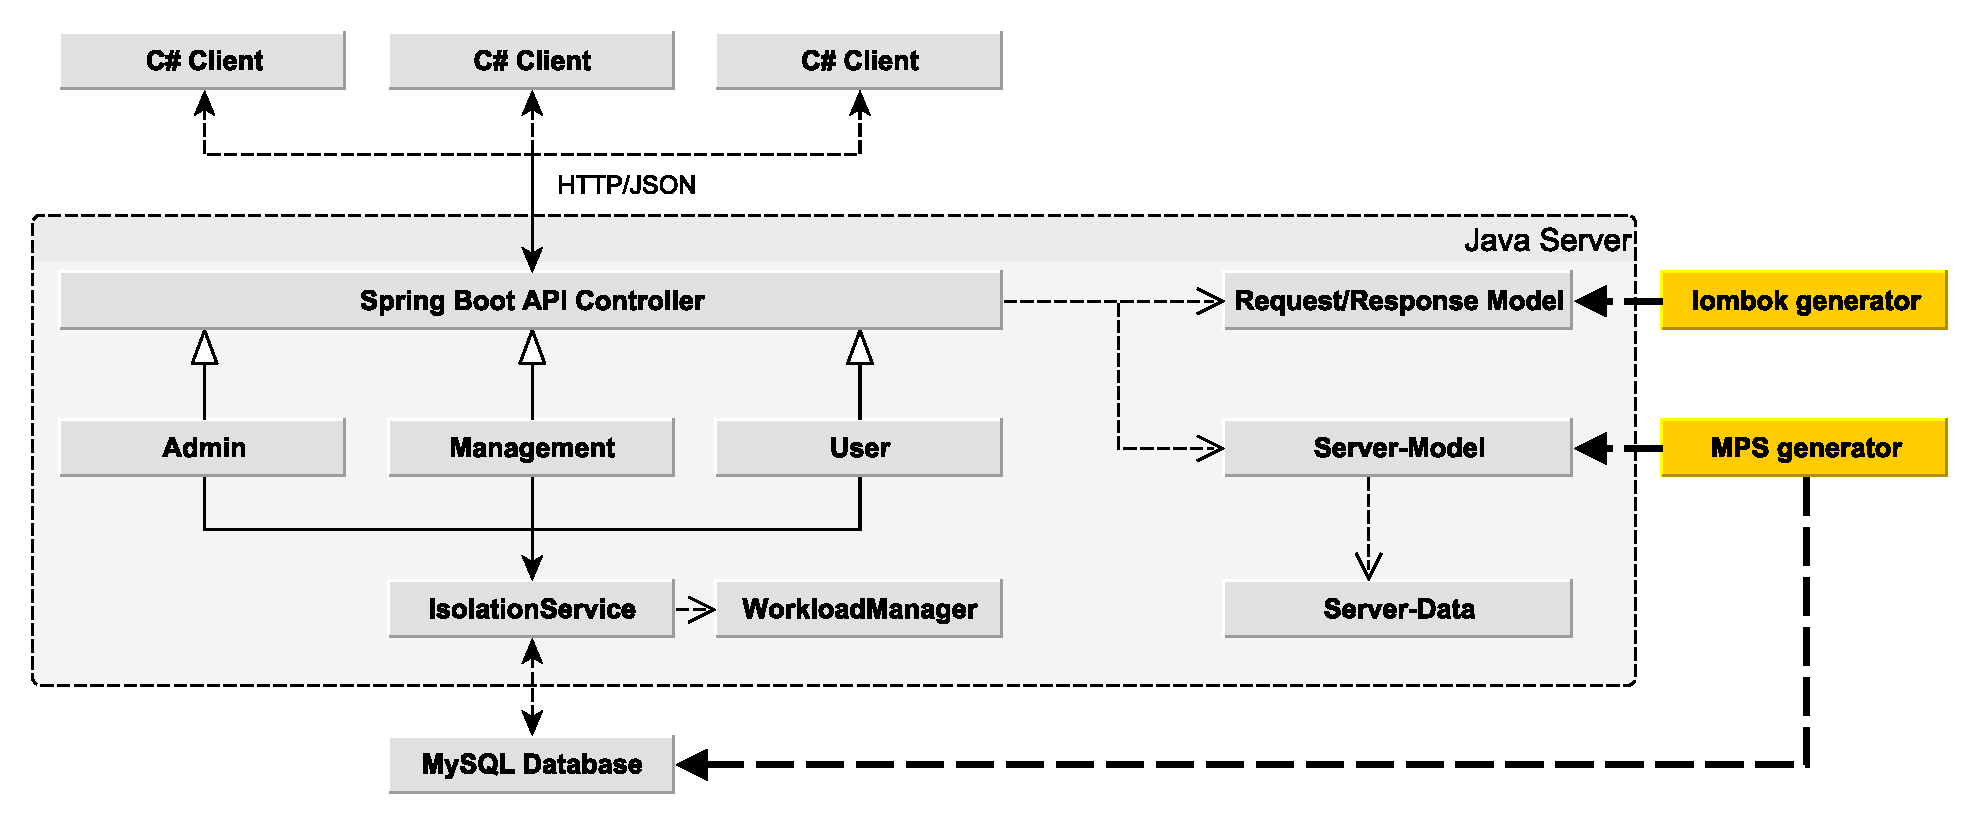
\includegraphics[width=\textwidth]{images/big-picture}
\caption{The final project architecture following the integration of Lombok.}
\label{fig:architecture-with-lombok}
\end{figure}

In the prototype, the \inlinecode{@Data} annotation was utilized to generate getter and setter methods for each field. This annotation was applied to all \gls{a:rrm} classes in the \gls{g:cms} prototype, reducing the amount of boilerplate code that needed to be written. This enhancement in code maintainability was accomplished with minimal effort and proved to be a significant time-saver, allowing the development team to concentrate more on implementing the actual functionality. The example provided in \vref{lst:lombok-example} demonstrates the advantages of using Lombok.

\begin{figure}[H]
\begin{minipage}[t]{0.5\textwidth}
\begin{minted}[fontsize=\scriptsize,linenos]{java}
public class UserUpgradeReservationRequest {
    private Integer reservationId;
    private String email;
    public Integer getReservationId() {
        return this.reservationId;
    }
    public void setReservationId(Integer value) {
        this.reservationId = value;
    }
    public String getEmail() {
        return this.email;
    }
    public void setEmail(String value) {
        this.email = value;
    }
}
...
String email = request.getEmail(); // works
\end{minted}
\end{minipage}
\hfill
\begin{minipage}[t]{0.5\textwidth}
\begin{minted}[fontsize=\scriptsize,linenos]{java}
@Data
public class UserUpgradeReservationRequest {
    Integer reservationId;
    String email;
}
...
String email = request.getEmail(); // works
\end{minted}
\end{minipage}
\captionof{listing}{The same class before and after applying the \inlinecode{Data} annotation}
\label{lst:lombok-example}
\end{figure}

\Cref{lst:lombok-example} demonstrates the \inlinecode{UserUpgradeReservationRequest} class before and after applying the \inlinecode{Data} annotation. The \inlinecode{Data} annotation automatically generates getter and setter methods for each field, which are then utilized in the same manner as in the original, manually written class. The code in the \inlinecode{UserUpgradeReservationRequest} class is reduced from 16 lines to 5 lines, corresponding to a 69\% reduction in boilerplate code. This decrease in boilerplate code leads to a substantial improvement in the project's maintainability, as less code needs to be written and managed.

\section{Reflective Object Mapping}\label{sec:impl-reflective-object-mapping}

An optimization applied to the \gls{a:rrm} implementation involved the addition of the \inlinecode{ObjectX} (Object Extensions) class. \inlinecode{ObjectX} offers a suite of reflection-based methods for populating a response object based on a given \gls{a:mps}-generated data model instance. Utilizing reflection, the \inlinecode{ObjectX} class identifies shared properties with matching names and data types between the two classes. Subsequently, a new instance of the response class is created, and values are transferred from the data model instance to the response class instance. \Cref{lst:reflective-object-mapping-example} demonstrates this process.

\begin{listing}[H]
\begin{minted}[fontsize=\scriptsize,linenos,mathescape]{java}
@GetMapping("/list")
public ResponseEntity<GetMoviesResponse> listMovies() 
{
    return isolated(() -> 
    {
        GetMoviesResponse response = new GetMoviesResponse();
        response.setMovies(ObjectX.createFromMany(               // ObjectX usage$\label{lst:objectx:ln:usage}$
            CinemaService.getInstance().getMovieCache().values(), 
            GetMoviesResponseEntry.class));
        response.setSuccess(true);
        return new ResponseEntity<GetMoviesResponse>(response, HttpStatus.OK);
    });
}
\end{minted}
\vspace{-.5cm}
\caption{Example of a controller method using the \inlinecode{ObjectX} class to efficiently transform a data model instance to a response model instance.}
\label{lst:reflective-object-mapping-example}
\end{listing}

\Vref{lst:reflective-object-mapping-example} presents an example of the \inlinecode{MovieController} class utilizing the \inlinecode{ObjectX} class in \lref{lst:objectx:ln:usage} for the efficient conversion of a collection of \inlinecode{Movie} instances into a set of \inlinecode{GetMoviesResponseEntry} response model instances.

In combination with the lombok-annotated response model classes, the overhead associated with modeling \gls{a:json} \glspl{a:rrm} is minimized, leading to a substantial enhancement in development speed.

\section{Challenges and limitations}\label{sec:impl-challenges}

During development of the prototype, a number of challenges were encountered, some of which are discussed in this section.

\subsection{Inserting Default Values for \headercode{PriceCategories}}\label{sec:impl-challenges-price}

As per the data model defined in \cref{sec:cs-data-model}, the \inlinecode{PriceCategory} class owns a \inlinecode{price} attribute. This attribute, intended to be of type \inlinecode{Rational}, corresponds to the ticket price for a given \inlinecode{PriceCategory}. As the default values are not part of the data model, the \inlinecode{price} attribute must be initialized with a value before being accessed by the application. The goal was to eagerly initialize the \inlinecode{price} upon the server startup. To accomplish this, the guard clause illustrated in \cref{lst:price-category-initialization} was added to the main method of the \gls{g:cms}:

\begin{listing}[H]
\begin{minted}[fontsize=\scriptsize]{java}
@SpringBootApplication
public class Program 
{
    public static void main(String[] args) 
    {
        if (!PriceCategoryStalls.getInstance().getPrice().isPresent())
        {
            PriceCategoryStalls.getInstance().setPrice(new Rational(10));
            PriceCategoryBox.getInstance().setPrice(new Rational(12));
            PriceCategoryServiceBox.getInstance().setPrice(new Rational(16));
        }
        SpringApplication.run(Program.class, args);
    }
}
\end{minted}
\caption{Guard clause for initializing default values of price categories.}
\label{lst:price-category-initialization}
\end{listing}

\Cref{lst:price-category-initialization} demonstrates the initialization of \inlinecode{PriceCategory} instances with default values if they are unset. However, this attempt to initialize default values did not yield the expected results. Although the \inlinecode{PriceCategoryBox} and \inlinecode{PriceCategoryServiceBox} singleton instances were initialized correctly, the \inlinecode{PriceCategoryStalls} instance was not. Further testing revealed that the first price category to be initialized would always fail, while subsequent attempts to initialize the corresponding price category would also prove unsuccessful. Other price categories could be initialized correctly, but the first price category would consistently fail. Due to time constraints, this issue could not be investigated further during development of the prototype. Consequently, the price attribute was temporarily removed from the data model, and offline price calculations were implemented based on the class type of a given \inlinecode{PriceCategory} instance.

Future work should thoroughly investigate this issue to determine the root cause and establish whether the bug originates in \gls{g:cms} or the generated data access layer.

\subsection{Inconsistent Database States and Missing Transactions}\label{subsec:missing-transactions}

The absence of database transactions generated by \gls{a:mps} significantly hindered the prototype development. Although concurrency issues were addressed using the isolation service described in \cref{sec:cs-isolation}, the lack of transactions prevented the data access layer from rolling back database changes in the event of an error. This issue manifested in the server application crashing randomly during subsequent data access operations, leading to considerable frustration during development. Consequently, until the error sources could be identified and resolved, the database was dropped and the \gls{a:mps} generator re-run each time the server was restarted during development. This practice resulted in a substantial increase in development time, as test data had to be re-entered every time the server was restarted.

Future work should prioritize extending the \gls{a:mps} generator to create accurate transactional data access code before deploying the prototype in a production environment.

\pagebreak

\section{Requirement validation}
\label{sec:ProjectReview}

The proposed conceptual solution was implemented in a pre-production prototype of the \gls{g:cms} and tested against the requirements identified in \cref{sec:requirements}. The results of the requirement validation are presented in \vref{tab:requirement-validation-results}.

\renewcommand{\arraystretch}{1.25}
\begin{table}[H]
    \centering
    \caption{Validation of requirements.}
    \label{tab:requirement-validation-results}
    \begin{tabular}{l|p{0.75\textwidth}}
        \toprule
        Requirement & Validation \\
        \midrule
        \ref{req:use-cases} & The \gls{g:cms} prototype covers all use-cases specified in \cref{sec:use-cases}. The use-cases described in \cref{apx:sec:use-cases} were tested successfully. \\ \hline
        \ref{req:model-requirements} & The data model was mostly implemented in accordance with the model requirements specified in \cref{apx:ch:extended-analysis} (see \cref{sec:cs-data-model}). Due to technical limitations the current version of the prototype does not implement the \inlinecode{price} attribute in the \inlinecode{PriceCategory} class (see \cref{sec:impl-challenges-price}). \\ \hline
        \ref{req:client-server} & The \gls{g:cms} implements a client–server model (see \cref{sec:infrastructure}, \cref{sec:cs-api}, and \ref{sec:cs-api-access}). \\ \hline
        \ref{req:database} & The \gls{g:cms} prototype uses a MySQL database for persistent data storage (see \cref{sec:infrastructure}). \\ \hline
        \ref{req:server} & The \gls{g:cms} server is implemented targeting Java 17. \gls{a:mps} and Project Lombok were used for code generation (see \cref{sec:infrastructure} and \ref{sec:impl-lombok}). \\ \hline
        \ref{req:mps} & \gls{a:mps} is used to generate the database schema and the data access layer (see \cref{sec:infrastructure} and \cref{sec:cs-data-mps}). \\ \hline
        \ref{req:mysql} & The \gls{g:cms} prototype uses a MySQL database for persistent data storage (see \cref{sec:infrastructure}). \\ \hline
        \ref{req:isolation} & The isolation service is ensures thread-safe database access (see \cref{sec:cs-isolation}). \\ \hline
        \ref{req:api} & \gls{g:spring} is used to implement a \gls{a:rest}ful \gls{a:json} \gls{a:api} (see \cref{sec:cs-api}). \\ \hline
        \ref{req:client-access} & The client is able to communicate with the server via the \gls{a:rest} \gls{a:api} (see \cref{sec:cs-api-access}). \\ \hline
        \ref{req:client-cli} & The client provides a \gls{a:cli} to allow user interaction with \gls{g:cms} (see \cref{sec:cs-cli}). \\ \hline
        \ref{req:client-firendly-cli} & The client extends the simple \gls{a:cli} with an additional ease-of-access layer for user interaction (see \cref{sec:cs-autocomplete}). \\ \hline
        \ref{req:client-portability} & The client application was implemented using C\# 11/.NET 7 and can be published without dependency on an external .NET runtime installation (see \cref{sec:cs-client}). \\
        \bottomrule
    \end{tabular}
\end{table}
\renewcommand{\arraystretch}{1}